\documentclass[11pt]{article} 
\usepackage[english]{babel}
\usepackage[utf8]{inputenc}
\usepackage[margin=0.5in]{geometry}
\usepackage{amsmath}
\usepackage{amsthm}
\usepackage{amsfonts}
\usepackage{amssymb}
\usepackage[usenames,dvipsnames]{xcolor}
\usepackage{graphicx}
%\usepackage[siunitx]{circuitikz}
\usepackage{tikz}
\usetikzlibrary{calc,arrows.meta}
\usepackage[colorinlistoftodos, color=orange!50]{todonotes}
\usepackage{hyperref}
\usepackage[numbers, square]{natbib}
\usepackage{fancybox}
\usepackage{epsfig}
\usepackage{soul}
\usepackage[framemethod=tikz]{mdframed}
\usepackage[shortlabels]{enumitem}
\usepackage[version=4]{mhchem}
\usepackage{multicol}

\usepackage{mathtools}
\usepackage{comment}
\usepackage{enumitem}
\usepackage[utf8]{inputenc}
\usepackage[linesnumbered,ruled,vlined]{algorithm2e}
\usepackage{listings}
\usepackage{color}
\usepackage[numbers]{natbib}
\usepackage{subfiles}
%\usepackage{tkz-berge}


\newtheorem{prop}{Proposition}[section]
\newtheorem{thm}{Theorem}[section]
\newtheorem{lemma}{Lemma}[section]
\newtheorem{cor}{Corollary}[prop]

\theoremstyle{definition}
\newtheorem{definition}{Definition}

\theoremstyle{definition}
\newtheorem{required}{Problem}

\theoremstyle{definition}
\newtheorem{ex}{Example}

\tikzset{
	vertex/.style={circle,draw,minimum size=16, inner sep=0pt,font=\normalsize},
	every node/.style={draw=none,rectangle,font=\scriptsize,outer sep=0pt,inner sep=2pt},
	directed/.style={arrows={-Stealth[length=7pt]},font=\small},
	caption/.style={text width=6cm,align=center,rectangle,draw}
}


\setlength{\marginparwidth}{3.4cm}
%#########################################################

%To use symbols for footnotes
\renewcommand*{\thefootnote}{\fnsymbol{footnote}}
%To change footnotes back to numbers uncomment the following line
%\renewcommand*{\thefootnote}{\arabic{footnote}}

% Enable this command to adjust line spacing for inline math equations.
% \everymath{\displaystyle}

% _______ _____ _______ _      ______ 
%|__   __|_   _|__   __| |    |  ____|
%   | |    | |    | |  | |    | |__   
%   | |    | |    | |  | |    |  __|  
%   | |   _| |_   | |  | |____| |____ 
%   |_|  |_____|  |_|  |______|______|
%%%%%%%%%%%%%%%%%%%%%%%%%%%%%%%%%%%%%%%

\title{
\normalfont \normalsize 
\textsc{CSCI 3104 Fall 2021 \\ 
Instructors: Profs. Grochow and Waggoner} \\
[10pt] 
\rule{\linewidth}{0.5pt} \\[6pt] 
\huge Midterm 1- Standard 11 \\
\rule{\linewidth}{2pt}  \\[10pt]
}
%\author{Your Name}
\date{}

\begin{document}
\definecolor {processblue}{cmyk}{0.96,0,0,0}
\definecolor{processred}{rgb}{200, 0, 0}
\definecolor{processgreen}{rgb}{0, 255, 0}
\DeclareGraphicsExtensions{.png}
\DeclareGraphicsExtensions{.gif}
\DeclareGraphicsExtensions{.jpg}

\maketitle


%%%%%%%%%%%%%%%%%%%%%%%%%
%%%%%%%%%%%%%%%%%%%%%%%%%%
%%%%%%%%%%FILL IN YOUR NAME%%%%%%%
%%%%%%%%%%AND STUDENT ID%%%%%%%%
%%%%%%%%%%%%%%%%%%%%%%%%%%
\noindent
Due Date \dotfill TODO \\
Name \dotfill \textbf{Didi Trifonova} \\
Student ID \dotfill \textbf{109388776} \\


\tableofcontents

\section{Instructions}
 \begin{itemize}
	\item The solutions \textbf{should be typed}, using proper mathematical notation. We cannot accept hand-written solutions. \href{http://ece.uprm.edu/~caceros/latex/introduction.pdf}{Here's a short intro to \LaTeX.}
	\item You should submit your work through the \textbf{class Canvas page} only. Please submit one PDF file, compiled using this \LaTeX \ template.
	\item You may not need a full page for your solutions; pagebreaks are there to help Gradescope automatically find where each problem is. Even if you do not attempt every problem, please submit this document with no fewer pages than the blank template (or Gradescope has issues with it).

	\item You \textbf{may not collaborate with other students}. \textbf{Copying from any source is an Honor Code violation. Furthermore, all submissions must be in your own words and reflect your understanding of the material.} If there is any confusion about this policy, it is your responsibility to clarify before the due date. 

	\item Posting to \textbf{any} service including, but not limited to Chegg, Discord, Reddit, StackExchange, etc., for help on an assignment is a violation of the Honor Code.

	\item You \textbf{must} virtually sign the Honor Code (see Section \ref{HonorCode}). Failure to do so will result in your assignment not being graded.
\end{itemize}


\section{Honor Code (Make Sure to Virtually Sign)} \label{HonorCode}

\begin{required}
\noindent 
\begin{itemize}
\item My submission is in my own words and reflects my understanding of the material.
\item I have not collaborated with any other person.
\item I have not posted to external services including, but not limited to Chegg, Discord, Reddit, StackExchange, etc.
\item I have neither copied nor provided others solutions they can copy.
\end{itemize}

%\noindent In the specified region below, clearly indicate that you have upheld the Honor Code. Then type your name. 
\end{required}

\begin{proof}[Agreed (Didi Trifonova).]
\end{proof}

\newpage
\section{Standard 11- Network Flows: Reductions}

\begin{required} \label{Problem2}
	In this problem we will consider a new reduction from finding a maximum matching in a unweighted, undirected bipartite graph to finding a maximum $(s,t)$-flow in a flow network.
	Let $G = (L \dot \cup R, E)$ be a bipartite graph with the vertices partitioned into $L$ and $R$.
	We construct an $(s,t)$-flow network $\mathcal{N} = (H, c, s,t)$ from $G$ as follows:
	\begin{itemize}
		\item Let $V(H) = V(G) \cup \{s,t\}$.
		\item For each edge $\{u,v\}$ in $E(G)$ with $u \in L$ and $v \in R$, add a directed edge $(u,v)$ to $E(H)$. For each of these edges, set $c(u,v) =1$.
		\item For each $v \in L$, add a directed edge $(s,v)$ to $E(H)$. For each of these edges, set $c(s,v) = 2$.
		\item For each $v \in R$, add a directed edge $(v,t)$ to $E(H)$. For each of these edges, set $c(v,t) = 1$.
	\end{itemize}
	
	\emph{To help you understand the reduction we have drawn in Figure~\ref{fig:H} an example of a bipartite graph and the resulting flow network. If you need to draw a graph as part of your answer you may copy and modify the tikzpictures or submit hand-drawn examples.}
	
	\begin{figure}[htbp]
		\centering
		
		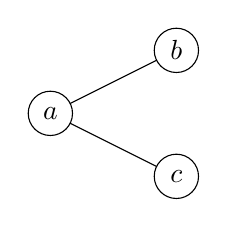
\begin{tikzpicture}[scale=1.6]
		\node[vertex] (a) at ($(0,0) + (1,0)$) {$a$};
		\node[vertex] (b) at ($(a) + (1,.5)$) {$b$};
		\node[vertex] (c) at ($(a) + (1,-.5)$) {$c$};
		
		\draw[] (a) to [edge label=] (b);
		\draw[] (a) to [edge label=] (c);
		\end{tikzpicture}
		\hspace{0.2\textwidth}
		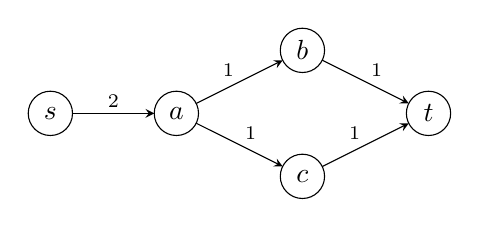
\begin{tikzpicture}[scale=1.6]
		\node[vertex] (s) at ($(0,0) + (1,0)$) {$s$};
		\node[vertex] (a) at ($(s) + (1,0)$) {$a$};
		\node[vertex] (b) at ($(a) + (1,.5)$) {$b$};
		\node[vertex] (c) at ($(a) + (1,-.5)$) {$c$};
		\node[vertex] (t) at ($(c) + (1,.5)$) {$t$};
		
		\draw[-stealth] (s) to [edge label=2] (a);
		\draw[-stealth] (a) to [edge label=1] (b);
		\draw[-stealth] (a) to [edge label=1] (c);
		\draw[-stealth] (b) to [edge label=1] (t);
		\draw[-stealth] (c) to [edge label=1] (t);
		\end{tikzpicture}
		
		\caption{A bipartite graph and the flow network we get by applying the above reduction. The number next to each edge represents the capacity of that edge.\label{fig:H}}
	\end{figure}


\noindent \textbf{Do the following.} Let $G(L \dot \cup R, E)$ be a bipartite graph, and let $\mathcal{N}$ the corresponding flow network obtained by applying the reduction.
\begin{enumerate}[label=(\alph*)]
\item Let $\mathcal{M}$ be a matching of $G$, where $|\mathcal{M}| = k$. Is it the case that $\mathcal{N}$ has a feasible flow $f$ where $\text{val}(f) = k$? If so, explain how to construct such a flow $f$ from $\mathcal{M}$. If not, carefully explain your reasoning.

\begin{proof}[Answer]
Yes you can create a flow on $\mathcal{N}$ such that $\text{val}(f) = k$. 
\begin{itemize}
    \item Start with all the edges in $\mathcal{N}$ that correspond to $\mathcal{M}$. They all have a capacity of 1 and no flow to start. 
    \item Create a flow augmenting path from s to t using one of the edges in $\mathcal{M}$. Push 1 unit along this path. 
    \item Repeat for each edge in $\mathcal{M}$. 
    \item Now you have pushed one unit of flow for each edge in $\mathcal{M}$.  
\end{itemize}

\end{proof}

%Include an Image: \includegraphics{ImageFileName}
%Include an Image and Rotate 90 degree: \includegraphics[angle=90]{ImageFileName}
%Include an Image, Rotate by 180 degrees, and scale by 50\% \includegraphics[scale=0.5, angle=90]{ImageFileName}



\vskip 50pt
\item Let $f^{\prime}$ be a feasible flow of $\mathcal{N}$ where for each edge $(u, v) \in E(H)$, $f^{\prime}(u, v)$ is an integer. Suppose that $\text{val}(f^{\prime}) = k$. Does the existence of $f^{\prime}$ imply that there is a matching $\mathcal{M}$ of size $k$ in $G$? That is, can we necessarily recover a matching of size $k$ of $G$ from $f^{\prime}$?  If so, explain how to construct such a matching $\mathcal{M}$ from $f^{\prime}$. If not, give a counterexample.

\begin{proof}[Answer] $ $ \\
No, the existence of $f^{\prime} = k$ does not imply there is a matching of size k in G. Consider the example in figure 1 and let $f^{\prime} = 2$ which is also the max flow. However, the maximum matching of G is 1, therefore, $k$ cannot equal 2. 
\end{proof}

%Include an Image: \includegraphics{ImageFileName}
%Include an Image and Rotate 90 degree: \includegraphics[angle=90]{ImageFileName}
%Include an Image, Rotate by 180 degrees, and scale by 50\% \includegraphics[scale=0.5, angle=90]{ImageFileName}

\end{enumerate}
\end{required}

%%%%%%%%%%%%%%%%%%%%%%%%%%%%%%%%%%%%%%%%%%%%%%%%%%
\end{document} % NOTHING AFTER THIS LINE IS PART OF THE DOCUMENT



